\chapter{Suchen und Sortieren}
\section{Lineare Suche}
\label{sec:lineareSuche}
Die Lineare Suche ist der einfachste Suchalgorithmus überhaupt.
Bei ihr wird solange ein Element nach dem anderen durchlaufen, bis ein Element mit dem gesuchten Schlüssel angetroffen wird.
Die lineare Suche hat eine Laufzeit von $\mathcal{O}(n)$ (n ist die Anzahl der Elemente der Liste) und kann sowohl auf sortierte als auch unsortierte Listen angewendet werden. 
\begin{lstlisting}[language=java, caption={Beispielimplementierung in Java}]
public static int lineareSuche(int gesucht, int[] daten) {
    for (int i = 0; i < daten.length; i++)
        if (daten[i] == gesucht)
            return i;
    return -1;
}
\end{lstlisting}

\section{Binäre Suche}
\label{sec:binaereSuche}
Die binäre Suche ist ein Algorithmus, der in einem Array sehr effizient ein gesuchtes Element findet bzw. eine zuverlässige Aussage über das Fehlen dieses Elementes liefert.
Voraussetzung ist, dass die Elemente in dem Array entsprechend sortiert sind.

Dazu wird immer das mittlere Element eines Felds überprüft.
Ist das Element gleich dem gesuchten Element ist die Suche beendet.
Ansonsten wird geprüft ob das Element kleiner als das gesuchte Element ist, dann muss sich das Element in der vorderen Hälfte befinden, ansonsten in der hinteren.
Dadurch wird der Suchbereich Schritt für Schritt halbiert bis das gesuchte Element gefunden ist oder nur noch eine Element vorhanden ist.

Für \(n=2^{k}\) lässt sich das Verhalten bei erfolgloser Suche als vollständiger Binärbaum darstellen.
Jeder Knoten entspricht ein Vergleich mit einem mittleren Feldelement.
Jedes Blatt entspricht einem Vergleich in einem Array der Länge 1, daher besitzt der Baum \(n\) Blätter.
\begin{figure}[htbp]
	\begin{center}
	\tikzstyle{end} = [circle, minimum width=4pt,fill, inner sep=0pt]
		\begin{tikzpicture}[sibling distance=5mm]
		\Tree [
		  . \node[end]{};
		      [. \node[end]{}; 
			    [.\node[end]{};
				  [. \node[end](a){}; ]
				  [. \node[end]{}; ]
			    ]
			    [. \node[end]{};
				  [. \node[end]{}; ]
				  [. \node[end]{}; ]
			    ]
		      ]
		      [. \node[end]{};
			    [.\node[end]{};
				  [. \node[end]{}; ]
				  [. \node[end]{}; ]
			    ]
			    [. \node[end]{};
				  [. \node[end]{}; ]
				  [. \node[end](z){}; ]
			    ]
		      ]
		]
		\draw[thick,decorate,decoration={brace,amplitude=12pt,mirror}] ($(a)+(-.2,0)$) -- ($(z)+(.2,0)$) node[midway, yshift=-20pt]{n};
		\end{tikzpicture}
	\end{center}
	\label{img:BinaerBaum}
	\caption{Einfacher Binärbaum}
\end{figure}
In einem vollständigen Binärbaum mit genau \(n=2^{k}\) Blättern besitzt jeder Pfad von der Wurzel zu einem Blatt die Länge \(k=\log_{2}n\).
Falls die Suche erfolgreich ist, ist die Laufzeit entsprechend kürzer.
Die Laufzeit der binären Suche liegt daher in \(\mathcal{O}(\log_{2}n)\).

\subsubsection{Induktionsbeweis}
\label{Beweis:BinaerBaum}
Behauptung: Ein vollständiger Binärbaum der Tiefe \(d\) besitzt genau \(2^{d}\) Blätter.
\begin{description}
 \item[\(d=0\)] Ein vollständiger Binärbaum der Tiefe 0 besitzt \(1=2^{0}\) Blätter.
	\item[\(d\rightarrow d+1\)] Wenn wir in einem vollständigen Binärbaum der Tiefe \(d+1\) die Wurzel entfernen, erhalten wir zwei vollständige Binärbäume der Tiefe \(d\).
			Diese besitzen nach Induktionsvorraussetzung jeweils genau \(2^{d}\) Blätter.
			Daraus folgt, dass der Binärbaum der Tiefe \(d+1\) genau \(2 \cdot 2^{d} = 2^{d+1}\) Blätter besitzt.
\end{description}

\subsubsection{Rekursionsgleichung}
Eine alternative Möglichkeit die Laufzeit des Algorithmuses zu bestimmen ist es die Rekursionsgleichung zu lösen.
Seien \(n=2^{k}\) und \(V(n)\) die Anzahl, die die binäre Suche mit dem gesuchten Wert ausführt.
So gilt bei erfolgloser Suche:

\begin{eqnarray*}
	V(1) &=& 1 \\
	V(n) &=& 1+ V(\frac{n}{2}) \\
	&=& 1+1+V(\frac{n}{4}) \\
	&=& 1+1+1+V(\frac{n}{8}) = 3 +V(\frac{n}{2^{3}}) \\
	&=& k+V(\frac{n}{2^{k}}) = \log(n) + V(\frac{n}{n})\\
	&=& \log(n) + V(1) \in \mathcal{O}(\log n)
\end{eqnarray*}

\subsubsection{Alternative Herrleitung}
Eine weitere Alternative Herrleitung geht über die Herrleitung einer Schleife:
\[ \textrm{Anzahl Schleifendurchläufe} \cdot \textrm{Aufwand pro Schleife} \]
\[ \mathcal{O}(k) \cdot \mathcal{O}(1) = \mathcal{O}(k) = \mathcal{O}(\log n) \]

\section{Binäre Suchbäume}
Um auch in dynamischen Datenstrukturen zu suchen, lassen sich Suchbäume verwenden.
Ein Suchbaum ist ein Binärbaum in dem gilt: Jeder in einem Knoten gespeicherte Wert ist größer als alle Knoten im linken Teilbaum und kleiner als alle Knoten im rechten Teilbaum.
\begin{figure}[htbp]
	\begin{center}
		\begin{tikzpicture}
		\Tree [
			.5
			[.3
				[.2 ]
				[.4 ]
			]
			[.8
				[.6 ]
				[.9 ]
			]
		]
		\end{tikzpicture}
	\end{center}
	\label{img:SuchBaum}
	\caption{Beispiel für einen Suchbaum}
\end{figure}
Folgende Funktionen sind nötig:
\begin{description}
	\item[Suchen nach einem Wert] Das wird der Suchbaum, beginnend an der Wurzel, rekursiv durchgesucht.
		Die Laufzeit liegt bei \(\mathcal{O}(n)\) für einen linear entarteten Baum und \(\mathcal{O}(\log n)\) für einen vollständigen Baum.
	\item[Wert hinzufügen] Dazu wird der Baum wie oben durchsucht und ein Blatt mit dem neuen Wert hinzugefügt falls der Wert noch nicht vorhanden ist.
		Die Laufzeit ist gleich der des durchsuchens eines Baumes.
	\item[Suchbaum aufbauen] Dazu kann mehrfach die obrige Funktion aufgerufen werden.
		Jedoch kann dabei ein unbalancierter Baum entstehen.
		Es gibt einen Algorithmus der einen optimalen Suchbaum aufbaut.
	\item[Wert entfernen] Es werden im allgemeinen zwei Fälle unterschieden:
		\begin{description}
			\item[einfacher Fall] Der zu entfernende Knoten hat keine oder genau einen Nachfolger
			\item[schwieriger Fall] Knoten besitzt zwei Nachfolger.
				Eine einfache Lösung ist es, den zu entfernenden Knoten mit dem kleinsten Knoten im rechten Unterbaum zu ersetzen.
				Dazu wird der Knoten mit minimalen Wert im rechten Unterbaum gesucht und durch einen rekursiven Aufruf entfernt und als eine Wurzel angehängt.
		\end{description}
\end{description}

\begin{figure}[htbp]
	\begin{center}
		\subfloat[Ausgangssuchbaum]{
			\begin{tikzpicture}
			\tikzset{ n/.style={draw=none} }
			\Tree [
				.5
				[.2
					\edge[n];[.{} ]
					[.4 
						[.3 ]
						\edge[n];[.{} ]
					]
				]
				[.8
					[.6
						\edge[n];[.{} ]
						[.7 ]
					]
					[.10
						[.9 ]
						[.11 ]
					]
				]
			]
			\end{tikzpicture}
		}
		\hspace{1cm}
		\subfloat[Resultat]{
			\begin{tikzpicture}
			\tikzset{ n/.style={draw=none} }
			\Tree [
				.6
				[.2
					\edge[n];[.{} ]
					[.4 
						[.3 ]
						\edge[n];[.{} ]
					]
				]
				[.8
					[.7 ]
					[.10
						[.9 ]
						[.11 ]
					]
				]
			]
			\end{tikzpicture}
		}
	\end{center}
	\label{img:SuchBaumAdd}
	\caption{Beispiel für das entfenen eines Wertes aus einem Suchbaum}
\end{figure}

Mit einer Grammatik lässt sich ein Binärbaum darstellen:
\[\textrm{BTree} \rightarrow \textrm{empty} \:|\: \textrm{node Btree Btree}\]
Zum Beispiel entspricht die Grammatik ``node(node empty empty) empty'' dem Baum
\begin{figure}[htbp]
	\begin{center}
	\tikzstyle{end} = [circle, minimum width=4pt,fill, inner sep=0pt]
		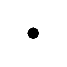
\begin{tikzpicture}[sibling distance=5mm]
			\Tree [. \node[end]{};
				[. \node[end]{};
					[. \node[end]{};
					]
					[. \node[end]{};
					]
				]
				[. \node[end]{};
				]
				];
		\end{tikzpicture}
	\end{center}
\end{figure}


\section{Hashing}
Gegeben sei eine Menge \(U\) von potentiellen Schlüsseln und eine Menge \(S \subseteq U\) von zu verwaltenden Schlüsseln.
Hashing ist geeignet, wenn \(|S|\) deutlich kleiner \(|U|\) ist und sich \(|S|\) nicht stark ändert.
Beispiel:
\begin{itemize}
	\item U \ldots alle möglichen ISBN-Nummern
	\item S \ldots tatsächlich in einer Buchhandlung vorkomenden ISBN-Nummern
\end{itemize}

Wir verwenden eine Hashfunktion \(h: U \rightarrow T\), die eine Hashtabelle \(T\) abbildet.
Ein Beispiel für eine Hashfunktion könnte \(h(s) = s \mod m\) sein, wenn \(m \leq |T|\) ist.
\(m\) sollte dabei eine Primzahl sein.
\begin{figure}[htbp]
	\begin{center}
		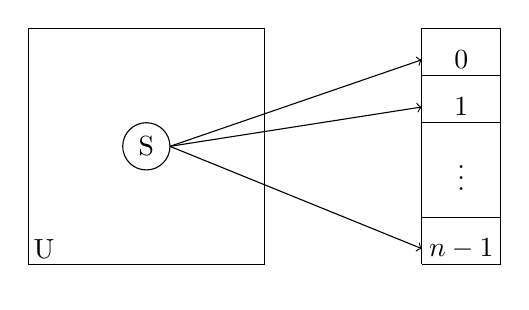
\begin{tikzpicture}[every node/.style={circle,inner sep=0pt}]
			\draw (0,0) -- (3,0) -- (3,3) -- (0,3) -- (0,0);
			\draw (1.5,1.5) circle [radius=.3] node {S};
			\draw (.2,.2) node {U};
			\draw (5,0) -- (6,0) -- (6,3) -- (5,3) -- (5,0);
			\draw (5.5,.2) node {\(n-1\)};
			\draw (5.5,2.6) node {0};
			\draw (5.5,2) node {1};
			\draw (5.5,1.2) node {\(\vdots\)};
			\draw (5,2.4) -- (6,2.4);
			\draw (5,1.8) -- (6,1.8);
			\draw (5,.6) -- (6,.6);
			\draw [->] (1.8,1.5) -- (5,2.6);
			\draw [->] (1.8,1.5) -- (5,2);
			\draw [->] (1.8,1.5) -- (5,.2);
		\end{tikzpicture}
	\end{center}
	\label{img:Hashfunktion}
	\caption{Hashfunktion die auf ein Array abbildet}
\end{figure}

Dabei können allerdings Kollisionen (mehre Schlüssel besitzen den gleichen Hashwert) auftretten.
Dies soll durch das folgende Beispiel verdeutlicht werden:
In einer Hashtabelle mit \(m=100\) Einträgen werden \(k\) zufällige Schlüssel eingetragen.
Wir nehmen an, dass die Hashfunktion gut streut und die Werte der Hashfunktion gleichmäßig verteilt sind.
Ab wann ist die Wahrscheinlickeit für eine Kollision \(\geq 0,5\)?
\begin{eqnarray*}
	P(Kollesion) &=& 1-(\textrm{kleine Kollesion}) \\
				&=& 1-1\cdot \frac{99}{100} \cdot \frac{98}{100} \cdot \ldots \cdot \frac{100-k+1}{100} > \frac{1}{2} \\
				&\Leftrightarrow& k \geq 13
\end{eqnarray*}
Allgemein ist bei etwa \(\sqrt{2m}\) vielen Einträgen mit einer Kollesion zu rechnen.

Die einfachste Art der Kollisionsbehandlung ist das Hashing mit Verkettung.
Dabei ist jedes Element der Hashtabelle eine Liste.
\begin{figure}[htbp]
	\begin{center}
		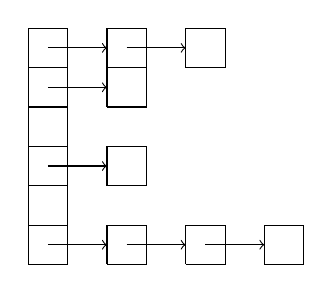
\begin{tikzpicture}[every node/.style={circle,inner sep=0pt}]
			\draw (0,0) -- (.5,0) -- (.5,3) -- (0,3) -- (0,0);
			\draw (0,.5) -- (.5,.5);
			\draw (0,1) -- (.5,1);
			\draw (0,1.5) -- (.5,1.5);
			\draw (0,2) -- (.5,2);
			\draw (0,2.5) -- (.5,2.5);
			\draw [->] (.25,.25) -- (1,.25);
			\draw (1,0) -- (1.5,0) -- (1.5,.5) -- (1,.5) -- (1,0);
			\draw [->] (1.25,.25) -- (2,.25);
			\draw (2,0) -- (2.5,0) -- (2.5,.5) -- (2,.5) -- (2,0);
			\draw [->] (2.25,.25) -- (3,.25);
			\draw (3,0) -- (3.5,0) -- (3.5,.5) -- (3,.5) -- (3,0);
			\draw [->] (.25,1.25) -- (1,1.25);
			\draw (1,1) -- (1.5,1) -- (1.5,1.5) -- (1,1.5) -- (1,1);
			\draw [->] (.25,2.25) -- (1,2.25);
			\draw (1,2) -- (1.5,2) -- (1.5,2.5) -- (1,2.5) -- (1,2);
			\draw [->] (.25,2.75) -- (1,2.75);
			\draw (1,2.5) -- (1.5,2.5) -- (1.5,3) -- (1,3) -- (1,2.5);
			\draw [->] (1.25,2.75) -- (2,2.75);
			\draw (2,2.5) -- (2.5,2.5) -- (2.5,3) -- (2,3) -- (2,2.5);
		\end{tikzpicture}
	\end{center}
	\label{img:HashVerkettung}
	\caption{Hashing mit Verkettung; alle Daten, deren Schlüssel auf denselben Hashwert führen, werden in die entsprechende Liste eingetragen}
\end{figure}

Der Belegungsfaktor einer Hastabelle mit  \(n\) Elementen ist \(\beta = \frac{n}{m}\).
Man kann zeigen, dass die mittlere Länge der Überlaufliste \(\beta\) ist.
Daraus ergibt sich die mittlere Anzahl Suchschritte \(1+\beta\).

\subsubsection{Dynamische Größenänderung}
Um die Suchzeit und den Platzbedarf gering zu halten, muss der Belegungsquotient begrenzt sein.
Eine einfache Möglichkeit ist es das beim Überschreiten eines Schwellwertes für \(\beta\) (typisch \(\beta = \frac{3}{4}\)) alle Einträge in eine größere Hashtabelle kopiert werden.
Entsprechend beim Unterschreiten eine Schwellwertes in eine kleinere Hashtabelle.
Mit einer amortisierten Analyse lässt sich zeigen, dass sich der amortisierte Aufwand (d.h. wir verteilen den Aufwand zum Kopieren auf alle vorherigen Hashoperationen) für die Hashtabelle dann in \(\mathcal{O}(1)\) liegt.


\section{Sortieren}

\begin{shaded}
  \noindent
  \textbf{Satz.:} In einem Binärbaum mit mind. \(2^{k}\) Blättern gibt es einen Pfad der Länge \(k\).
\end{shaded}
Der Satz lässt sich mit Hilfe des Beweises im Kapitel \ref{Beweis:BinaerBaum} indirekt beweisen.
\[a \rightarrow b \equiv \neg b \rightarrow \neg a\]
Dies würde bedeuten wenn alle Pfade kürzer als \(k\) sind, besitzt der Baum \(< 2^{k}\) Blätter, was zu einem Widerspruch führt.

Ein Sortierverfahren, dass ausschließlich paarweise Vergleiche verwendet, lässt sich als Binärbaum darstellen.
In jedem Knoten wird ein Vergleich \(a \leq b\) ausgeführt.
Jedes Blatt entspricht einer sortierten Folge,
Jede sortierte Folge entspricht einer Permutation der Ausgangsfolge.
Der Binärbaum besitzt daher \(n!\) Blätter und deshalb einen Pfad der Länge \(\log_{2}n!\).
Ein Sortierverfahren, dass paarweise Vergleiche ausführt besitzt daher eine Worst-Case Laufzeit in \(\Omega(\log_{2}n!) = \Omega(n\log_{2}n) - \mathcal{O}(n))\).
\begin{figure}[htbp]
	\begin{center}
	\tikzstyle{end} = [circle, minimum width=4pt,fill, inner sep=0pt]
		\begin{tikzpicture}[sibling distance=5mm]
			\Tree [. 1:2
				\edge node[auto=right]{\(\leq\)};
				[.2:3
					\edge node[auto=right]{\(\leq\)}; \(\{1,2,3\}\)
					\edge node[auto=left]{\(>\)};
					[.1:3
						\edge node[auto=right]{\(\leq\)}; \(\{1,3,2\}\)
						\edge node[auto=left]{\(>\)}; \(\{3,1,2\}\)
					]
				]
				\edge node[auto=left]{\(>\)}; 
				[.1:3
					\edge node[auto=right]{\(\leq\)}; \(\{2,1,3\}\)
					\edge node[auto=left]{\(>\)};
					[.2:3
						\edge node[auto=right]{\(\leq\)}; \(\{2,3,1\}\)
						\edge node[auto=left]{\(>\)}; \(\{3,2,1\}\)
					]
				]
				];
\end{tikzpicture}
	\end{center}
	\label{img:Suchnaum}
	\caption{Entscheidungsbaum für 3 Elemente (\(\{1,2,3\}\))}
\end{figure}

Naive Verfahren wie Bubbelsort haben ein Laufzeit von \(\mathcal{O}(n^2)\).
Ein besseres Verfahren ist Quicksort.
Die Laufzeit ist schwierig zu berechnen da die Teillisten unterschiedliche Längen besitzen.
Ein ähnliches Verfahrenist Mergesort, welches nachfolgend behandelt wird.


\subsection{Mergesort}
Mergesort betrachtet die zu sortierenden Daten als Liste und zerlegt sie in kleinere Listen, die jede für sich sortiert werden.
Die sortierten kleinen Listen werden dann zu größeren Listen zusammengefügt, bis wieder eine sortierte Gesamtliste erreicht ist.
Das Verfahren arbeitet bei Arrays in der Regel nicht in-place.

\begin{figure}[htbp]
	\begin{center}
	\tikzstyle{end} = [circle, minimum width=4pt,fill, inner sep=0pt]
		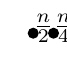
\begin{tikzpicture}[sibling distance=5mm]
			\Tree [. \node[end]{};
				\edge node[auto=right]{\(\frac{n}{2}\)};
				[. \node[end]{};
					\edge node[auto=right]{\(\frac{n}{4}\)};
					[. \node[end]{};
						\node[end]{};
						\node[end]{};
					]
					\edge node[auto=left]{\(\frac{n}{4}\)};
					[. \node[end]{};
						\node[end]{};
						\node[end]{};
					]
				]
				\edge node[auto=left]{\(\frac{n}{2}\)};
				[. \node[end]{};
					\edge node[auto=right]{\(\frac{n}{4}\)};
					[. \node[end]{};
						\node[end]{};
						\node[end]{};
					]
					\edge node[auto=left]{\(\frac{n}{4}\)};
					[. \node[end]{};
						\node[end]{};
						\node[end]{};
					]
				]
				];
		\end{tikzpicture}
	\end{center}
	\caption{Darstellung als Binärbaum}
	\label{fig:Mergesort}
\end{figure}
Das Verhalten lässt sich wie in Abbildung \ref{fig:Mergesort} als Baum darstellen.
Vereinfacht nehmen wir \(n=2^{k}\) an.

Beim Zusammenfügen fällt der Aufwand \(\mathcal{O}((\textrm{linke Liste}) + (\textrm{rechte Liste}))\) an.
Auf jeder Ebene ist das \(\mathcal{O}(n)\).
Zum halbieren der Liste fällt jeweils der Aufwand \(\mathcal{O}(n)\) an.
Pro Ebene insgesammt also \(\mathcal{O}(n)\).
Der Baum besitzt \(n\) Blätter, die Liste der der Länge 1 entsprechen (Mehr als n Listen der Länge 1 können nicht erzeugt werden \(\curvearrowright\) n Blätter).
Der Baum hat daher die Tiefe \(\log_{2}n\) (d.h. k).
Die Laufzeit liegt daher in in \(\mathcal{O}(n \cdot  \log n)\).
Auch die mittlere Laufzeit von Quicksort liegt in \(\mathcal{O}(n \log n)\).

\subsubsection{Übung}
Bestimmen Sie die Laufzeit durch eine Rekursionsgleichung.
\(V(n)\) ist dabei die Anzahl der Vergleiche.
\begin{eqnarray*}
	V(1) &=& 0 \\
	V(n) &=& \underbrace{n}_{\textrm{Zusammenfügen}} + \underbrace{V(\frac{n}{2}) + V(\frac{n}{2})}_{\textrm{Sortieren}} = n + 2V(\frac{n}{2}) \\
	V(n+1) &=& 2n + 4V(\frac{n}{4}) \\
		&\vdots&	\\
		&=& k \cdot n + 2^{k} \cdot V(\frac{n}{2^{k}})	\\
		&=&n \cdot \log n
\end{eqnarray*}

\subsubsection{Worst Case Laufzeit von Quicksort}
Im Worst Case wird das Pivotelement stehts so gewählt, dass es das größte oder das kleinste Element der Liste ist.
Dies ist etwa der Fall, wenn als Pivotelement stets das Element am Ende der Liste gewählt wird und die zu sortierende Liste bereits sortiert vorliegt.
\begin{eqnarray*}
	V(n) &=& n-1 + V(n-1)	\\
		 &=& n-1 + n-2 + V(n-2)	\\
		 &=& \sum \limits_{k=1}^{n-1} k + V(0) = \frac{n(n-1)}{2} \in \mathcal{O}(n^{2})
\end{eqnarray*}

\subsection{Heap Sort}
Ein Heap ist ein Binärbaum, in dem jeder Knoten einen kleineren (Min-Heap) bzw. einen größeren (Max-Heap) Wert besitzt als seine Nachfolger (Abbildung \ref{fig:MinHeap}).
\begin{figure}[htbp]
	\begin{center}
		\begin{tikzpicture}
		\Tree [
			.1
			[.2
				[.3 ]
				[.8 ]
			]
			[.6
				[.9 ]
				[.7 ]
			]
		]
		\end{tikzpicture}
	\end{center}
	\caption{Beispiel für einen Min-Heap}
	\label{fig:MinHeap}
\end{figure}
Ein Linksbaum ist ein Heap, der effiziente Heapoperationen ermöglicht.
Wir stellen Binär\-bäume als erweiterte Binär\-bäume dar, so dass jeder innere Knoten genau 2 Nachfolger hat  (Abbildung \ref{fig:BinaerBaumExtendet}).
\begin{figure}[htbp]
	\begin{center}
 		\subfloat[Binärbaum]{
			\trimbox{-.5cm 0cm -.5cm 0cm}{
				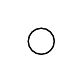
\begin{tikzpicture}[sibling distance=5mm]
					\tikzset{ n/.style={draw=none} }
					\tikzstyle{end} = [circle,draw, minimum width=4pt]
					\Tree [
						.\node[end]{};
						[.\node[end]{}; ]
						\edge[n];[.{} ]
					]
				\end{tikzpicture}
			}
		}
		\hspace{1cm}
		\subfloat[erweiterte Binärbaum]{
			\trimbox{-1cm 0cm -1cm 0cm}{
				\begin{tikzpicture}[sibling distance=5mm]
						\tikzstyle{end} = [circle, minimum width=4pt,fill, inner sep=0pt]
						\Tree [
							.\node[state]{};
								[.\node[state]{};
									[.\node[end]{}; ]
									[.\node[end]{}; ]
								]
							.\node[state]{};
								[.\node[end]{}; ]
						]
				\end{tikzpicture}
			}
		}
	\end{center}
	\caption{Erweiterung eines Binärbäumes}
	\label{fig:BinaerBaumExtendet}
\end{figure}
Für einen Knoten \(x\) ist \(s(x)\) die Länge des Pfades zu einem Blatt.
Ein Binärbaum ist ein Linksbaum wenn für jeden inneren Knoten \(x\) gilt:
\[s(\textrm{linker Nachfolger}(x)) \geq s(\textrm{rechter Nachfolger}(x)) \]

\subsubsection{Eigenschaften}
\begin{enumerate}
	\item \label{itm:first} \(s(root)\) ist die Länge des Pfades ganz rechts.
	\item \label{itm:second} Für die Anzahl \(n\) der inneren Knoten  gilt:
		\[ n\geq \sum \limits_{k=0}^{s(root)-1} 2^{k} = 2^{s(root)}-1\]
	\item Aus \ref{itm:first}, \ref{itm:second} folgt: Die Länge des Pfades ganz rechts liegt in \(\mathcal{O}(\log n)\).
\end{enumerate}

\subsubsection{Operationen}
\begin{itemize}
	\item put
	\item removeMin
	\item init
	\item merge
\end{itemize}

\subsubsection{Merge-Operation für einen Linksbaum}
Wir suchen den Baum mit dem kleineren Wurzelwert und betrachten dessen rechten Teilbaum.
Merge wird wird rekursiv aufgerufen für diesen rechten Teilbaum und den anderen Baum.

\begin{tabular}{M{.45\textwidth}M{.45\textwidth}}
% 0. Zeile
	\multicolumn{2}{l}{\rule{0pt}{5ex}Gegebene Bäume:}
	\\
% 1. Zeile
	\begin{tikzpicture}[sibling distance=5mm]
		\Tree [
			.\node[state]{4};
			[.\node[state]{6};
				[.\node[state]{8}; ]
				[.\node[state]{6}; ]
			]
			[.\node[state]{8};	]
		]
	\end{tikzpicture}
	&
	\begin{tikzpicture}[sibling distance=5mm]
		\Tree [
			.\node[state]{3};
			[.\node[state]{5};
				[.\node[state]{7}; ]
				\edge[none];[.{} ]
			]
			[.\node[state]{6}; 	]
		]
	\end{tikzpicture}
	\\
		\multicolumn{2}{l}{\rule{0pt}{5ex}Begin der Rekursion:}
	\\
% 2. Zeile
	\begin{tikzpicture}[sibling distance=5mm]
		\Tree [
			.\node[state]{4};
			[.\node[state]{6};
				[.\node[state]{8}; ]
				[.\node[state]{6}; ]
			]
			[.\node[state]{8}; ]
		]
		\end{tikzpicture}
	&
	\begin{tikzpicture}[sibling distance=5mm]
		\Tree [.\node[state]{6}; ]
	\end{tikzpicture}
	\\
	\multicolumn{2}{l}{\rule{0pt}{5ex}Nächster Schritt:}
	\\
% 3. Zeile
	\begin{tikzpicture}[sibling distance=5mm]
		\Tree [.\node[state]{8}; ]
	\end{tikzpicture}
	&
	\begin{tikzpicture}[sibling distance=5mm]
		\Tree [.\node[state]{6}; ]
	\end{tikzpicture}
\end{tabular}


Hier endet die Rekursion, da der rechte Teilbaum des Baumes mit der kleineren Wurzel leer ist.
Unter dem Baum mit der kleinen Wurzel wird rechts der andere Baum gehängt.
Wenn dabei die Linksbaumeigenschaft verletzt wird, werden die Teilbäume vertauscht.

\begin{tabular}{M{.35\textwidth}M{.2\textwidth}M{.35\textwidth}}
% 1. Zeile
	\multicolumn{2}{l}{Da dies kein Linksbaum ist,}
	&
	\multicolumn{1}{l}{ergibt sich}\\
% 2. Zeile
	\begin{tikzpicture}[sibling distance=8mm]
		\Tree [.\node[state](1){6};
			[.\node[EndPoint](2){}; ]
			[.\node[state](3){8}; 
				[.\node[EndPoint]{}; ]
				[.\node[EndPoint]{}; ]
			]
		]
		\node[node distance=5mm,right of=1]{1};
		\node[node distance=5mm,left of=2]{0};
		\node[node distance=5mm,right of=3]{1};
	\end{tikzpicture}
	&
	&
	\begin{tikzpicture}[sibling distance=5mm]
		\Tree [.\node[state]{6};
			[.\node[state]{8}; ]
			\edge[none];[.{} ]
		];
	\end{tikzpicture}
	\\
% 3. Zeile
	\multicolumn{2}{l}{\rule{0pt}{5ex}Nächster Schritt: Merge von}
	&
	\multicolumn{1}{l}{ergibt}\\
% 4. Zeile
	\begin{tikzpicture}[sibling distance=5mm]
		\Tree [.\node[state]{4};
			[.\node[state]{6};
				[.\node[state]{8}; ]
				[.\node[state]{6}; ]
			]
			\edge[none];[.{} ]
		];
	\end{tikzpicture}
	& 
	\begin{tikzpicture}[sibling distance=5mm]
		\Tree [.\node[state]{6};
			[.\node[state]{8}; ]
			\edge[none];[.{} ]
		];
	\end{tikzpicture}
	&
	\begin{tikzpicture}[sibling distance=5mm]
		\Tree [.\node[state]{4};
			[.\node[state]{6};
				[.\node[state]{8}; ]
				[.\node[state]{6}; ]
			]
			[.\node[state]{6};
				[.\node[state]{8}; ]
					\edge[none];[.{} ]
			]
		];
	\end{tikzpicture}	\\
% 5. Zeile
	\multicolumn{2}{l}{\rule{0pt}{5ex}Nächster Schritt: Merge von}
	&
	\multicolumn{1}{l}{ergibt}\\
% 6. Zeile
	\begin{tikzpicture}[sibling distance=5mm]
		\Tree [.\node[state]{4};
			[.\node[state]{6};
				[.\node[state]{8}; ]
				[.\node[state]{6}; ]
			]
			[.\node[state]{6};
				[.\node[state]{8}; ]
					\edge[none];[.{} ]
			]
		];
	\end{tikzpicture}
	&
	\begin{tikzpicture}[sibling distance=5mm]
		\Tree [.\node[state]{3};
			[.\node[state]{5};
				[.\node[state]{7}; ]
				\edge[none];[.{} ]
			]
			\edge[none];[.{} ]
		];
	\end{tikzpicture}
	&
	\begin{tikzpicture}[sibling distance=3mm]
		\Tree [.\node[state]{3};
			[.\node[state]{5};
				[.\node[state]{7}; ]
				\edge[none];[.{} ]
			]
			[.\node[state]{4};
				[.\node[state]{6};
					[.\node[state]{8}; ]
					[.\node[state]{6}; ]
				]
				[.\node[state]{6};
					[.\node[state]{8}; ]
						\edge[none];[.{} ]
				]
			]
		];
	\end{tikzpicture}	\\
% 7. Zeile
	\multicolumn{3}{l}{\rule{0pt}{5ex}{Da dieser Baum die Linksbaumeigenschaft verletzt muss er umgeformt werden}} \\
% 8. Zeile
	\begin{tikzpicture}[sibling distance=3mm]
		\Tree [.\node[state]{3};
			[.\node[state]{4};
				[.\node[state]{6};
					[.\node[state]{8}; ]
					[.\node[state]{6}; ]
				]
				[.\node[state]{6};
					[.\node[state]{8}; ]
						\edge[none];[.{} ]
				]
			]
			[.\node[state]{5};
				[.\node[state]{7}; ]
				\edge[none];[.{} ]
			]
		];
	\end{tikzpicture}
	&
	&
\end{tabular}

\newpage
\subsubsection{Laufzeitanalyse der Operation Merge}
Für die Laufzeitanalyse sind bei der Implentierung folgende Schritte notwendig:
\begin{itemize}
	\item Erzeugen der Teilbäume vor jeden Rekursionsschritt: \(\mathcal{O}(1)\)
	\item Zusammenbau der Teilbäume nach der Rekursion (nur wenn die s-Werte zwischengespeichert werden): \(\mathcal{O}(1)\)
	\item Anzahl der rekursiven Aufrufe: Die Rekursion endet, wenn der rechte Teilbaum nur aus einem Knoten besteht.
		Bei jedem rekursiven Aufruf verkleinert sich einer der rechten Teilbäume.
		Die Laufzeit beträgt daher \(\mathcal{O}(\log n)\)
\end{itemize}
Mit Hilfe der Merge Operation können alle anderen Heap-Operationen realisiert werden:
\begin{description}
	\item[put] merge(heap, \(<\)neuer Knoten\(>\))
	\item[removeMin] Wurzel enfernen und die zwei neuen Teilbäume mergen
	\item[init] Mit Hilfe von put in der Zeit \(\mathcal{O}(n \log n)\). Es gibt einen besseren Algorithmus für init welcher eine Laufzeit von \(\mathcal{O}(n)\) besitzt.
\end{description}

Mergesort kann man durch folgenden Algorithmus darstellen:
\begin{itemize}
	\item Max-Heap aufbauen: \(\mathcal{O}(n)\)
	\item n-mal die Funktion removeMax aufrufen und Elemente am Kopf einer Liste anfügen: \(\mathcal{O}(n \log n)\)
\end{itemize}
Damit ist die Laufzeit \(\mathcal{O}(n \log n)\), welche gleich der Average Laufzeit von Quicksort ist.
Es gibt ebenfalls eine In-Place-Implentierung die dem Heap als Array darstellt.
Damit hat HeapSort alle Vorteile von Quicksort und Mergesort ohne deren Nachteile zu besitzten.